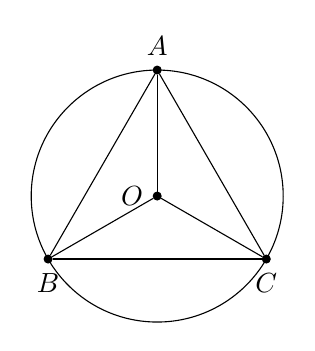
\begin{tikzpicture}
[scale =0.05,>=stealth,point/.style = {draw, circle, fill = black, inner sep = 1pt},]
\def\rad{32}
\coordinate [point, label={left: $O$ }] (O) at (27.712,16);
\draw (O) circle (\rad);
\node (B) at (0,0)[point,label=below :$B$] {};
\node (C) at (55.42,0)[point,label=below :$C$] {};
\node (A) at (27.712,48)[point,label=above :$A$] {};
\draw (A)--(C);
\draw (O)--(C);
\draw (O)--(B);
\draw (A)--(O);
\draw (A)--(B);
\draw (B)--(C);

\end{tikzpicture}
